%%
%% Author: Davidov
%% 23.04.2018
%%

\documentclass[12pt,a4paper]{book}

%underline emph
\renewcommand{\emph}[1]{\textbf{#1}}

%packages for math symbols
\usepackage{amsmath}
\usepackage{amssymb}
\usepackage{textcomp}
\usepackage{mathpartir}
\usepackage{stmaryrd}
\usepackage{mathtools}

% package for graphs
\usepackage{tikz}
\usetikzlibrary{graphs}
\usetikzlibrary{positioning}
\usetikzlibrary{automata}
\usetikzlibrary{arrows,decorations.pathmorphing,backgrounds,positioning,fit,petri}

% package for urls
\usepackage{hyperref}

%package for using
\usepackage{graphicx}

%package for proof and other theorem environments
\usepackage{amsthm}

%this package provides a pendant to "itemize" with better spacing - use compactitem
\usepackage{paralist}

%supports some nice characters with mathscr
\usepackage{mathrsfs}

%enables better support for tables
\usepackage{array}
\usepackage{multirow}

% various theorems, numbered by section
\newtheorem{theorem}{Theorem}[section]
\newtheorem{lemma}[theorem]{Lemma}
\newtheorem{proposition}[theorem]{Proposition}
\newtheorem{corollary}[theorem]{Corollary}
\newtheorem{definition}[theorem]{Definition}
\newtheorem{example}[theorem]{Example}

\newenvironment{remark}[1][Remark]{\begin{trivlist}
\item[\hskip \labelsep {\bfseries #1}]\end{trivlist}}

\newcolumntype{C}[1]{>{\parbox[c][#1][c]{0cm}{}}c<{}}

%some own commands
\newcommand{\expspace}[1]{#1-EXPSPACE/$_{\raise.17ex\hbox{$\scriptstyle\sim$}}$}
\newcommand{\exptime}[1]{#1-EXPTIME/$_{\raise.17ex\hbox{$\scriptstyle\sim$}}$}

%set of own commands
%\newcommand{\hcat}{\rotatebox{90}{$\ominus$}}
\newcommand{\hcat}{
\mathchoice{\rotatebox{90}{$\displaystyle\ominus$}}
{\rotatebox{90}{$\ominus$}}
{\rotatebox{90}{$\scriptstyle\ominus$}}
{\rotatebox{90}{$\scriptscriptstyle\ominus$}}}
\newcommand{\vcat}{
\mathchoice{\raisebox{1pt}{$\displaystyle\ominus$}}
{\raisebox{1pt}{$\ominus$}}
{\raisebox{0.5pt}{$\scriptstyle\ominus$}}
{\raisebox{0.2pt}{$\scriptscriptstyle\ominus$}}}
\newcommand{\plusinbox}{
\setlength\fboxsep{0pt}
\setlength{\fboxrule}{0.00001pt}
\text{ \framebox[8pt]{+} }
\setlength\fboxsep{3pt}
\setlength{\fboxrule}{0.4pt}
}
\newcommand{\mirroredL}{
\resizebox{0.31cm}{!}{\tiny\begin{tabular}[b]{C{0.4cm}|C{0.4cm}|}
\cline{2-2}
&\tabularnewline
\hline
\multicolumn{1}{|c|}{}&\tabularnewline
\hline
\end{tabular}}\normalsize}
%document information
\title{Capturing Bisimulation-Invariant Complexity Classes by Polyadic Higher-Order Fixpoint Logic}

\author{David Kronenberger}

\makeatletter
\def\maketitle{%

\begin{center}
\textbf{\textsf{\Huge \@title}}\\
\vspace{2cm}
{\Large by\\
\@author\\
\vspace{2.5cm}
Prof. Dr. Martin Lange, Advisor
}\\
\vspace{2.5cm}
A thesis submitted in partial fulfillment\\
of the requirements for the\\
Degree of Master of Science\\
in Computer Science\\
\vspace{2cm}
UNIVERSITY OF KASSEL\\
Hesse, Germany\\
\vspace{1cm}
\@date
\end{center}
}

\begin{document}

\maketitle
\thispagestyle{empty}

\pagebreak

\cleardoublepage
\vspace*{30\baselineskip}
\hbox to \textwidth{\hrulefill}
\par
\hbox to \textwidth{I declare that I have developed and written the enclosed thesis entirely}
\hbox to \textwidth{by myself, and have not used sources or means without declaration in the text.}
\vspace{0.9cm}
\hbox{\textbf{Kassel, \today}}
\vspace{0.6cm}

\hbox{\ldots\ldots\ldots\ldots\ldots\ldots\ldots\ldots\ldots\ldots\ldots\ldots}~\\
\hbox{\hspace*{1cm}(\textbf{David Kronenberger})} %center name with hspace

\thispagestyle{empty}

\pagebreak

\tableofcontents
\thispagestyle{empty}
\pagebreak

\setcounter{page}{1}
\chapter{Introduction}\label{ch:introduction}

The higher order cases of PHFL and a restriction called
tail-recursive for this higher order cases we are interested to compare with the in
Section~\ref{sec:descriptiveComplexity} introduced complexity classes \exptime{$k$} and \expspace{$k$}.

\chapter{Preliminaries}
\label{ch:preliminaries}
This chapter introduces all necessary definitions to prove that PHFL$^k =$~\exptime{$k$} and
PHFL$^{k+1}_{tail} =$~\expspace{$k$}. The notions are mainly from~\cite{immerman1999descriptive},
~\cite{papadimitriou1994complexity},~\cite{otto1999bisimulation},~\cite{freireMartins2011descriptive}
and~\cite{lange2014capturing}.

We assume that the reader is already familiar with basic notions of first order logic and 
computational complexity. In the first section we define a special kind of graphs called LTS and 
define some properties on it. Also in this section we define queries with special forms of queries. 
In the next section we give some information on fixpoints that are used the section that follows. 
There is defined the logic PHFL. In Section~\ref{sec:descriptiveComplexity} we present the 
descriptive complexity and the complexity clases \exptime{$k$} and \expspace{$k$}. In the last section we define the higher-order logic and combinations with LFP and PFP.

%%
%% Author: Davidov
%% 16.05.2018
%%

\subsection{Bisimulation Invariance}\label{subsec:bisimulationInvariance}

First of all, we need the definition of \textit{labeled transition systems}. A labeled transition system is a graph
with labeled vertices and edges. Formally, it is the following.

\begin{definition}
    \label{definition:lts}
    A quintuple $\mathcal{T} = (Q, \Sigma, P, \Delta, \nu)$ is called a \emph{labeled transition system} (\emph{LTS}),
    where
    \begin{compactitem}
        \item $Q$ is a set of states,
        \item $\Sigma$ is a finite set of actions,
        \item $P$ is a finite set of propositions,
        \item $\Delta \subseteq Q \times \Sigma \times Q$ is the labeled transition relation and
        \item $\nu: Q \rightarrow 2^P$ is a function that maps each state to a set of propositions.
    \end{compactitem}
\end{definition}

For all $q_1, q_2 \in Q$ and all $a \in \Sigma$ we write $q_1 \overset{a}{\rightarrow} q_2$ for $(q_1, a, q_2) \in
\Delta$.

\begin{example}
    As mentioned above, LTS can be seen as a graph with labeled vertices and edges. One example for a LTS is
    $\mathcal{T} = (\{0, 1, 2, 3, 4\}, \{a, b\}, \{p, q\}, \Delta, \nu)$
\begin{center}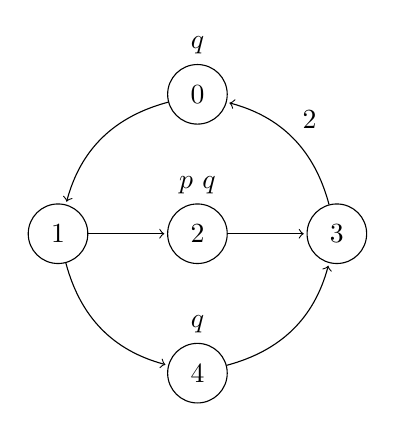
\begin{tikzpicture}[]
                  \node [place] (w1) [label=above:$q$] {0};
                  \node [place] (c1) [below=of w1,label=above:$p~q$] {2};
                  \node [place] (s) [below=of c1,label=above:$q$] {4};
                  \node [place] (e1) [left=of c1] {1}
                  edge [pre,bend left] (w1)
                  edge [post,bend right] (s)
                  edge [post] (c1);
                  \node [place] (l1) [right=of c1] {3}
                  edge [pre] (c1)
                  edge [pre,bend left] (s)
                  edge [post,bend right] node[auto, swap] {2} (w1);
\end{tikzpicture}
\end{center}
\end{example}

On this systems or rather on the states of the systems it is possible to define relations. The
following relation describes those states that have the same behaviour. For this, let be $\mathcal{T}_1 = (Q_1,
\Sigma_1, P_1, \Delta_1, \nu_1)$ and $\mathcal{T}_2 = (Q_2, \Sigma_2, P_2, \Delta_2, \nu_2)$ two LTSs.

\begin{definition}
    A \emph{bisimulation} is a binary relation $R \subseteq Q_1 \times Q_2$ that fulfills for all $(q_1, q_2) \in R$
    \begin{compactitem}
        \item $\nu_1 (q_1) = \nu_2 (q_2)$,
        \item for all $a_1 \in \Sigma_1$ and all $q_1' \in Q_1$, if $q_1 \overset{a_1}{\rightarrow} q_1' \in
        \Delta_1$, then there is a state $q_2' \in Q_2$ with $a_1 \in \Sigma_2$, $q_2
        \overset{a_1}{\rightarrow} q_2' \in \Delta_2$ and $(q_1', q_2') \in R$ and
        \item for all $a_2 \in \Sigma_2$ and all $q_2' \in Q_2$, if $q_2 \overset{a_2}{\rightarrow} q_2' \in
        \Delta_2$, then there is a state $q_1' \in Q_1$ with $a_2 \in \Sigma_1$, $q_1
        \overset{a_2}{\rightarrow} q_1' \in \Delta_1$ and $(q_1', q_2') \in R$.
    \end{compactitem}
    We call two states $q_1 \in Q_1$, $q_2 \in Q_2$ \emph{bisimilar}, noted as $(\mathcal{T}_1, q_1) \sim
    (\mathcal{T}_2, q_2)$, if there
    is a bisimulation $R$ such that $(q_1, q_2) \in R$.
\end{definition}

Furthermore, we can describe properties of LTS. \textit{Queries} are one way to describe these properties. A query
is a mapping that associates a LTS $\mathcal{T} = (Q, \Sigma, P, \Delta, \nu)$ to a subset
$M^{\mathcal{T}}$ of $Q \times \dots \times Q$. Remark, that any isomorphism $f: \mathcal{T} \simeq
\mathcal{T}'$ is also an isomorphism of $M^{\mathcal{T}}$ and $M^{{\mathcal{T}}'}$.

\begin{definition}
    \label{definition:query}
    A function $\mathcal{Q} : \mathscr{T} \rightarrow \mathscr{Q} \times \dots \times \mathscr{Q}, [\mathcal{T}]_\simeq
    \mapsto M^{\mathcal{T}}$ is called a
    \emph{$r$-adic query},
    where
    \begin{compactitem}
        \item $\mathscr{T}$ is the set of all equivalence classes of LTS relative to isomorphism,
        \item $\mathscr{Q}$ is the set of all equivalence classes of sets of states relative to isomorphism,
        \item $[\mathcal{T}]_\simeq = ([Q^\mathcal{T}]_\simeq, [\Sigma^\mathcal{T}]_\simeq, [P^\mathcal{T}]_\simeq,
        [\Delta^\mathcal{T}]_\simeq, [\nu^\mathcal{T}]_\simeq) \in \mathscr{T}$ is the equivalence class of LTS
        $\mathcal{T}$ relative to isomorphism and
        \item $M^{\mathcal{T}} \in \mathcal{P}([Q^\mathcal{T}]_\simeq \times \dots \times [Q^\mathcal{T}]_\simeq)$ is a
        set of tuples of states from $[\mathcal{T}]_\simeq$, i.e. $(q_1, \dots, q_r) \in M^{\mathcal{T}}$ with $q_1,
        \dots, q_r \in [Q^\mathcal{T}]_\simeq$.
    \end{compactitem}
\end{definition}

The queries defined in Definition~\ref{definition:query} can be categorized. Here we are interested in two of these
categories. The first category is called \textit{bisimulation invariant}. This category describes those queries that
can't distinguish bisimilar states. In~\cite{otto1999bisimulation} this property is defined over so called
\textit{Kripke structures}. A Kripke structure
is a transition system. Remark, that transition systems  have only one type of actions. This means the edges of the
graph haven't labels.

\begin{definition}
    \label{definition:bisimulationInvariant}
    Let $\mathcal{T}$, $\mathcal{T}'$ be two LTSs with $\mathcal{T} = (Q, \Sigma, P, \Delta, \nu)$
    and $\mathcal{T}' = (Q', \Sigma', P', \Delta', \nu')$. Furthermore, let be $(q_1, \dots, q_r) \in Q \times \dots
    \times Q$ and $({q_1}', \dots, {q_n}') \in Q' \times \dots \times Q'$.

    A query $\mathcal{Q}$ is called \emph{bisimulation invariant} if $(\mathcal{T}, q_i) \sim (\mathcal{T}', q_i')$
    for all $1 \leq i \leq r$ implies that $(q_1, \dots, q_r) \in \mathcal{Q}([\mathcal{T}]_\simeq)$ iff $({q_1}',
    \dots, {q_n}') \in \mathcal{Q}([\mathcal{T}']_\simeq)$.
\end{definition}

The second category of a query tells us which complexity class a query belongs to.

\begin{definition}
    \label{definition:queryBelongsToComplexityClass}
    Let $\mathcal{T}$ be a LTS with $\mathcal{T} = (Q, \Sigma, P, \Delta, \nu)$ and $(q_1, \dots, q_{r}) \in Q \times
    \dots \times Q$.

    A query $\mathcal{Q}$ belongs to complexity class $\mathcal{C}$ if there is an algorithm in $\mathcal{C}$ for
    deciding on input $(\mathcal{T}, (q_1, \dots, q_{r}))$ whether $(q_1, \dots, q_{r}) \in \mathcal{Q}
    ([\mathcal{T}]_\simeq)$.
\end{definition}

This definition leads us to the next chapter and the definitions for descriptive complexity.

%%
%% Author: Davidov
%% 16.05.2018
%%

\section{Fixpoints}\label{sec:fixpoints}

To define the polyadic higher-order fixpoint logic and the higher-order logic with least and partial fixpoints, we examine fixpoints in general in this section. The first fixpoint we consider is the least fixpoint.

\begin{definition}
   Let $F\colon A \rightarrow A$ be an operator on a finite set $A$, then $x \in A$
   is called a \emph{fixpoint} of $F$ if $F(x) = x$. Let $x$ be a fixpoint of $F$ and $\sqsubseteq$ an partial order on $A$, then $x$ is called the \emph{least
   fixpoint} of $F$, abbreviated as $\mathit{LFP}$($F$), if for all other fixpoints $y$ of $F$ the condition $x
   \sqsubseteq y$ holds. A fixpoint $x$ is called the \emph{greatest fixpoint} if $y \sqsubseteq x$ for all fixpoints $y$ of $F$.
\end{definition}

From the Knaster-Tarski Theorem~\cite{tarski1955lattice} we know that if an operator $F\colon A \rightarrow 
A$ is monotone and $A$ is a complete lattice regarding to $\sqsubseteq$ then the least and greatest fixpoints of $F$ exists. $F$ is monotone if for all $x, y
 \in A$ if $x \sqsubseteq y$ then $F(x) \sqsubseteq F(y)$ holds.

\begin{example}
    \label{example:lfp} Let $\mathcal{T} = (Q, \Sigma, P, \Delta, v)$ be an LTS and $F: Q^2 \rightarrow Q^2$ an operator on $Q^2$ defined as 
\begin{align*}
    F(X) =\, &\{(q, p) \in Q^2 \mid v(q) \neq v(p)\}\, \cup \\&
    \{(q,p) \in Q^2 \mid \text{it exists } a\in\Sigma \text{ with } q\overset{a}{\rightarrow} q' \text{ such that for all } p' \in Q \\&\text{ it holds } p\overset{a}{\rightarrow} p' \text{ implies } (q', p') \in X\}\,\cup \\&\{(q,p) \in Q^2 \mid  \text{it exists } a\in\Sigma \text{ with } p\overset{a}{\rightarrow} p' \text{ such that for all } q' \in Q \\&\text{ it holds } q\overset{a}{\rightarrow} q' \text{ implies } (q', p') \in X\}
\end{align*}   
Then $LFP(F)$ represents all those pairs of states $(q, p)$ such that $q\not\sim p$.
\end{example}

The following theorem shows a possibility to calculate the least fixpoint of a monotone operator if the operating set is a complete lattice with respect to its order.

\begin{theorem}[Kleene Fixed-Point Theorem~\cite{stoltenberghHansen1994mathematical}]
\label{theorem:kleene}
Let $F: A \rightarrow A$ be a monotone operator on $A$ and $A$ regarding to $\sqsubseteq$ a complete lattice, then it exists a finite sequence $X_0, \dots, X_m$ such that the first part $X_0$ is the smallest element in $A$ with respect to $\sqsubseteq$, the $(i+1)$-th part $X_{i+1}$ is $F(X_i)$ and $X_m = X_{m+1}$.
\end{theorem}

Next, we define the partial fixpoint. Since the
$\mathit{LFP}$ restricts the operator to be monotone, the partial fixpoint need no restriction on the operator.

\begin{definition}
\label{definition:pfp}
    Let $F\colon A \rightarrow A$ be an operator on a finite set $A$, then the \emph{partial
    fixpoint} of $F$, abbreviated as $\mathit{PFP}$($F$), is defined as follows:
    \[\mathit{PFP}(F)\coloneqq\begin{cases}
               F^{i+1}(\varnothing)=F^i(\varnothing),  & \text{if such } i \in \{0,\dots,|A|\} \text{ exists}\\
               \varnothing, & \text{otherwise,}
    \end{cases}\]
    where $F^0(\varnothing) = \varnothing$, $F^1(\varnothing) = F(\varnothing)$, $F^2(\varnothing) = F(F(\varnothing))$, and so on.
\end{definition}

Note, that for monotone $F$ holds $\mathit{PFP}(F)$ equals $\mathit{LFP}(F)$. 


\begin{example}
\label{example:pfp}
Let $F: \mathcal{P}(\{1, \dots, n\}) \rightarrow  \mathcal{P}(\{1, \dots, n\})$ be an operator on $ \mathcal{P}(\{1, \dots, n\})$ defined as
\begin{align*}
	F(X) = \{x \in \{1, \dots, n\}\mid &\; x\in X \text{ and it exists } y \in \{1, \dots, n\} \text{ such that }\\ &\;y < x \text{ and } y\not\in X \text{ or } \\&\;x\not\in X \text{ and for all } y\in \{1,\dots, n\} \text{ holds if } \\&\;y<x \text{ then } y\in X\}. 
\end{align*}
If we see $X \in \mathcal{P}(\{1,\dots, n\})$ as a binary string $b$, where a $1$ at the $i$-th position means that $i$ is in $X$, then $F(X)$ returns the set $Y$ such that the binary string $b'$ of $Y$ is $b' = b+1\mod n$. Then $PFP(F)$ returns $\varnothing$ because for every $i$ it holds $F^i(\varnothing) \neq F^{i+1}(\varnothing)$.
\end{example}

%%
%% Author: Davidov
%% 16.05.2018
%%

\section{Polyadic Higher Order Fixpoint Logic}\label{sec:polyadichigherorderfixpointlogic}

In this section, we present a logic with name Polyadic Higher Order Fixpoint Logic, abbreviated with PHFL, that was
introduced by M. Lange and E. Lozes in~\cite{lange2014capturing}. It is defined over LTS (see
Definition~\ref{definition:lts}) and extends the polyadic modal $\mu$-calculus~\cite{otto1999bisimulation} with
higher order fixpoints like M. Viswanathan and R. Viswanathan it did with monadic case of modal
$\mu$-calculus~\cite{kozen1983results} in~\cite{viswanathan2004higher}. The logic of M. Viswanathan and R
.Viswanathan with name higher order fixed point logic is a combination of propositional logic, modal operators and
a simply typed $\lambda$-calculus with fixed point operators. The higher order cases of PHFL and a restriction called
tail-recursive for this higher order cases we are interested to compare with the in
Chapter~\ref{sec:descriptiveComplexity} introduced complexity classes \exptime{$k$} and \expspace{$k$}.

\subsection{PHFL Types}\label{subsec:phflTypes}

Before defining formulas of PHFL we need to introduce the PHFL types. These definitions are guided
by~\cite{viswanathan2004higher} and~\cite{lange2014capturing}.

\begin{definition}
    \emph{PHFL types} are given by the grammar
    \[\sigma, \tau \Coloneqq \bullet \mid \sigma^v \rightarrow \tau,\]
    where $v$ is called \textit{variance}. The \emph{variances} of PHFL are defined by the grammar
    \[v \Coloneqq + \mid - \mid 0.\]
\end{definition}

All types will be interpreted as a partially ordered sets. Partial orders are relations that are reflexive, transitive
and antisymmetric. Let $\mathcal{A} = (A, \leq_A)$ and $\mathcal{B} = (B, \leq_B)$ be two partial orders. Then
$\mathcal{A} \rightarrow \mathcal{B}$ is the partial order of monotone functions ordered pointwise, i.e.
\[\mathcal{A} \rightarrow \mathcal{B} = \{f\colon A\rightarrow B \mid \text{ for all } x,y \in A.\,x\leq_A y \text{
implies }
f(x)
\leq_B f(y)\}\]
and the ordering relation is given by
\[f \leq_{\mathcal{A}\rightarrow\mathcal{B}} g\text{ iff } \text{ for all } x\in \mathcal{A}.\,f(x) \leq_{\mathcal{B}} g
(x)\].

\begin{definition}
    Let $\mathcal{T} = (Q, \Sigma, P, \Delta, v)$ be a LTS and $d \in \mathbb{N}$ the dimension of PHFL,
    then $\llbracket\tau\rrbracket_\mathcal{T}$ the
    semantics
    of type $\tau$ is defined by $\tau$ as follows:
        \[\llbracket\tau\rrbracket_\mathcal{T}=
        \begin{cases}
            (\mathcal{P}(Q^d), \subseteq),  & \text{if }\tau = \bullet\\
            ((\llbracket\sigma_1\rrbracket_\mathcal{T})^v \rightarrow \llbracket\sigma_2\rrbracket_\mathcal{T}, \leq_{
            (\llbracket\sigma_1\rrbracket_\mathcal{T})^v \rightarrow \llbracket\sigma_2\rrbracket_\mathcal{T}}), &
            \text{if }\tau = \sigma_1^v\rightarrow \sigma_2,
        \end{cases}\]
    where for any partial order $\mathcal{A} = (A, \leq_A)$, $\mathcal{A}^v = (A, \leq_A^v)$ is a partial order
    with $\leq_A^+ = \leq_A$, $\leq_A^- = \{(a, b) \mid (b, a) \in \leq_A\}$ and $\leq_A^0 = \leq_A^+ \cap \leq_A^-$.
\end{definition}

The partial orders $\llbracket\tau\rrbracket_\mathcal{T}$ for any PHFL type $\tau$ are complete lattices. That means we
have meets and joins, denoted by $\sqcap_{\llbracket\tau\rrbracket_\mathcal{T}}$ and
$\sqcup_{\llbracket\tau\rrbracket_\mathcal{T}}$, and least and greatest elements, denoted by
$\bot_{\llbracket\tau\rrbracket_\mathcal{T}}$ and $\top_{\llbracket\tau\rrbracket_\mathcal{T}}$ for any subset of
$\llbracket\tau\rrbracket_\mathcal{T}$. This ensures that the least and greatest fixpoint over all monotone PHFL types
exist~\cite{tarski1955lattice}. See Chapter~\ref{subsec:hoPlusLfp} for further information about fixpoints.

\begin{definition}
    The \emph{maximal arity} $ma(\tau)$ and the \emph{order} $ord(\tau)$ of a PHFL type $\tau$ are defined
    inductively on
    $\tau$ as follows:
\[ma(\tau)=
\begin{cases}
    1, & \text{if }\tau = \bullet\\
    max(\{n\} \cup \{ma(\tau_i)\mid1,\dots,n\}), &
    \text{if }\tau = \tau_1\rightarrow\dots\rightarrow\tau_n\rightarrow\bullet
\end{cases}\]
\[ord(\tau)=
\begin{cases}
    0, & \text{if }\tau = \bullet\\
    max(\{1 + ord(\sigma_1), ord(\sigma_2)\}), & \text{if }\tau = \sigma_1 \rightarrow \sigma_2
\end{cases}\]
\end{definition}

Next, we want to define the syntax of PHFL formulas.

\subsection{PHFL Syntax}\label{subsec:phflSyntax}

\begin{figure}
    \caption{Derivation Rules for PHFL formulas.}
    \label{figure:phfl-typing-rules}
    \begin{mathpar}
        \Gamma \vdash \top \colon \bullet \and
        \Gamma \vdash p_i \colon \bullet \and
        \inferrule{\Gamma \vdash \Phi \colon \bullet}{\Gamma \vdash \langle a \rangle_i \Phi \colon \bullet} \and
        \inferrule{\Gamma \vdash \Phi \colon \bullet}{\Gamma \vdash \{\emph{i} \leftarrow \emph{j}\}\Phi \colon
        \bullet} \and
        \inferrule{\Gamma^-\vdash\Phi\colon \bullet}{\Gamma \vdash \neg \Phi \colon \bullet} \and
        \inferrule{\Gamma\vdash\Phi \colon \tau \\ \Gamma\vdash\Psi\colon \tau}{\Gamma \vdash \Phi \vee
        \Psi \colon  \tau} \and
        \inferrule{v \in \{+, 0\} }{\Gamma, X^v \colon\tau \vdash X\colon\tau} \and
        \inferrule{\Gamma,X^v\colon\sigma\vdash \Phi\colon\tau}{\Gamma\vdash \lambda (X^v \colon \tau)
        .\Phi\colon\sigma^v\rightarrow\tau} \and
        \inferrule{\Gamma,X^+ \colon \tau \vdash \Phi\colon\tau}{\Gamma \vdash \mu (X \colon\tau). \Phi\colon\tau} \and
        \inferrule{\Gamma\vdash \Phi\colon\sigma^+ \rightarrow \tau \\ \Gamma\vdash\Psi\colon\sigma}{\Gamma \vdash
        \Phi\,\Psi \colon \tau} \and
        \inferrule{\Gamma\vdash \Phi\colon\sigma^- \rightarrow \tau \\ \Gamma^-\vdash\Psi\colon\sigma}{\Gamma \vdash
        \Phi\,\Psi \colon \tau} \and
        \inferrule{\Gamma\vdash \Phi\colon\sigma^0 \rightarrow \tau \\ \Gamma \vdash \Psi\colon\sigma \\ \Gamma^-
        \vdash\Psi\colon\sigma}{\Gamma \vdash \Phi\,\Psi \colon \tau} \and
    \end{mathpar}
\end{figure}

\begin{definition}
    Let $P$ a set of propositions, $\Sigma$ a set of actions and $\mathcal{V} = \{X_1, X_2, \dots\}$ a countable
    infinite
    set of variables, then
    \emph{$d$-adic PHFL formulas} $\Phi, \Psi,\dots$ are defined by the grammar
    \begin{align*}
        \Phi,\Psi\Coloneqq&\top \mid p_i \mid \Phi \vee \Psi \mid \neg \Phi \mid \langle a \rangle_i \Phi \mid
        \{\emph{j}\,\} \Phi \mid X \mid \lambda (X^v\colon\tau).\Phi \mid \Phi\,\Psi\mid  \mu (X\colon\tau).\Phi
    \end{align*}
    where
    \begin{compactitem}
        \item $\emph{j} = (e(1), \dots, e(d))$ and $e: \{1, \dots, d\} \rightarrow \{1, \dots, d\}$,
        \item $i \in \{1, \dots, d\}$
        \item $v$ is a variance,
        \item $\tau$ is a type,
        \item $p \in P$,
        \item $a \in \Sigma$ and
        \item $X \in \mathcal{V}$.
    \end{compactitem}
\end{definition}

For convenience, we use some other further standard notations like $\Phi \wedge \Psi$, $[a]_i\Phi$, $\nu
X \colon \tau.\Phi$ or $\Phi \Leftrightarrow \Psi$. Note, that this logic is defined over LTS. The formulas are
often interpreted as a game played by two players moving pebbles along the transitions of an LTS. The two players
are called Prover and Refuter. So, $p_i$ can be interpreted as, the position of the $i$-th pebble fulfills
property $p$. $\langle a \rangle_i \Phi$ means, Prover has to move the $i$-th pebble along an $a$-transition and
check if there holds $\Phi$. With the formula $\{\emph{j}\,\} \Phi$ is mentioned, that all pebbles
are moved from Prover to the positions described by tuple $\emph{j}$ and after this $\Phi$ have to
be fulfilled. The player who has to move the pebbles changes on negations. $\lambda (X^v\colon\tau).\Phi$ is
interpreted as a function that expects arguments of $(\llbracket\tau\rrbracket_\mathcal{T})^v$. We see, that the
formulas also have types. For this, we have ensure that a formula is well-typed.

\begin{definition}
    Let $X_1, \dots, X_n$ variables, $\Phi$ a PHFL formula, $v_1, \dots, v_n$ variances and $\tau, \tau_1, \dots,
    \tau_n$ types, then $\Gamma = X_1^{v_1}\colon \tau_1, \dots X_n^{v_n} \colon \tau_n$ is
    called a \emph{type environment} and $\Gamma \vdash \Phi\colon\tau$
    is called a \emph{type judgement}. Let $\Gamma^- = X_1^{v_1^-}\colon \tau_1, \dots
    X_n^{v_n^-} \colon \tau_n$ be a type environment then $\Gamma^- = X_1^{v_1^-}\colon \tau_1, \dots
    X_n^{v_n^-} \colon \tau_n$, where $-^- = +$, $+^- = -$ and $0^- = 0$.
\end{definition}

A type judgment is called \textit{derivable} if it generates a derivation tree according to the rules of
Figure~\ref{figure:phfl-typing-rules}. This type system ensures that we do not create senseless formulas like
$\langle a \rangle_i p_j p_k$. Furthermore, it can order formulas with semantics and guarantees so monotonicity. A
formula $\Phi$ is called \textit{well-typed} if the type judgement $\emptyset \vdash \Phi:\tau$ is derivable for some
type $\tau$. Note, that we are here only interested in well-typed formulas. For those formulas where also the variable
types are obvious, we omit the type on the variables.

\subsection{PHFL Semantics}\label{subsec:phflSemantics}

\begin{figure}
    \caption{Semantics of PHFL formulas.}
    \label{figure:phfl-semantics}
    \begin{align*}
        \llbracket \Gamma \vdash \top \colon \bullet \rrbracket^\eta_\mathcal{T} =\,& Q^d\\
        \llbracket \Gamma \vdash p_i \colon \bullet \rrbracket^\eta_\mathcal{T} =\,& \{(q_1, \dots, q_d) \in Q^d \mid p \in v
        (q_i)\}\\
        \llbracket \Gamma \vdash \langle a \rangle_i \Phi \colon \bullet \rrbracket^\eta_\mathcal{T} =\,& \{(q_1,
        \dots, q_d) \in Q^d \mid \text{ it exists } \\& ({q'}_1, \dots, {q'}_d) \in \llbracket \Gamma \vdash \Phi \colon
\bullet \rrbracket^\eta_\mathcal{T} \text{ such that } \\&q_i \overset{a}{\rightarrow} {q'}_i \text{ and for all } j
        \neq
        i \text{ holds } q_j = {q'}_j\}\\
        \llbracket \Gamma \vdash \Phi \vee \Psi \colon \tau \rrbracket^\eta_\mathcal{T} =\,& \llbracket \Gamma \vdash \Phi
        \colon \tau \rrbracket ^\eta_\mathcal{T} \sqcup_\tau \llbracket \Gamma \vdash \Psi \colon \tau \rrbracket ^\eta_\mathcal{T}\\
        \llbracket \Gamma \vdash \neg \Phi \colon \bullet \rrbracket^\eta_\mathcal{T} =\,& Q^d \setminus \llbracket
        \Gamma^- \vdash \Phi
        \colon \bullet \rrbracket ^\eta_\mathcal{T}\\
        \llbracket \Gamma \vdash \{\emph{j}\} \Phi \colon \bullet \rrbracket^\eta_\mathcal{T} =\,&
        \{\{(q_1, \dots, q_d) \in Q^d \mid \\ &(q_{j_1}, \dots, q_{j_d}) \in \llbracket \Gamma \vdash \Phi
        \colon \bullet
        \rrbracket ^\eta_\mathcal{T}\}\\
        \llbracket \Gamma, X \colon \tau \vdash X \colon \tau \rrbracket^\eta_\mathcal{T} =\,& \eta(X)\\
        \llbracket \Gamma \vdash \mu (X \colon \tau).\,\Phi \colon \tau \rrbracket^\eta_\mathcal{T} =\,&
        \bigsqcap\,_{\llbracket\tau\rrbracket_\mathcal{T}} \{\mathcal{X} \in \llbracket \tau \rrbracket_\mathcal{T}
        \mid \\
        &\llbracket \Gamma, X^+ \colon \tau \vdash \Phi \colon \tau \rrbracket^{\eta[X \mapsto \mathcal{X}]}_\mathcal{T}
        \leq_{\llbracket \tau \rrbracket_\mathcal{T}} \mathcal{X}\}\\
        %\llbracket         \Gamma
 %       \vdash
  %      \lambda X^+ \colon \tau.\Phi \colon \tau \rrbracket ^\eta_\mathcal{T}\\
        \llbracket \Gamma \vdash \lambda (X^v \colon \sigma).\,\Phi \colon \sigma^v \rightarrow \tau \rrbracket
        ^\eta_\mathcal{T} =\,& F \in \llbracket \sigma^v \rightarrow \tau \rrbracket_\mathcal{T} \text{ such that for
        all }
        \mathcal{X} \in \llbracket \sigma \rrbracket_\mathcal{T}.\, \\
        &F(\mathcal{X}) = \llbracket \Gamma, X^v \colon \sigma \vdash \Phi \colon \tau \rrbracket^{\eta[X \mapsto
        \mathcal{X}]}_\mathcal{T}\\
        \llbracket \Gamma \vdash \Phi\,\Psi \colon \tau \rrbracket^\eta_\mathcal{T} =\,& \llbracket \Gamma \vdash \Phi
        \colon \sigma
        ^v \rightarrow \tau \rrbracket ^\eta_\mathcal{T}(\llbracket \Gamma \vdash \Psi \colon \sigma \rrbracket ^\eta_\mathcal{T})
    \end{align*}
\end{figure}

To define the semantics of PHFL formulas we need a mapping $\eta$ that associates to each variable an element of its
type semantics, i.e. $\eta(X) \in \llbracket\tau\rrbracket_\mathcal{T}$ for $X$ of type $\tau$. Let $\Phi$ be a
well-typed formula of type $\tau$, $\mathcal{T}$ a LTS and $\eta$ a variable mapping, then the semantics
$\llbracket\Gamma \vdash \Phi\colon \tau \rrbracket^\eta_\mathcal{T}$ are defined inductively on $\Phi$ which maps to
an element of $\llbracket\tau\rrbracket_\mathcal{T}$ as explained in Figure~\ref{figure:phfl-semantics}.
Note, that $\eta[X \mapsto \mathcal{X}]$ is a mapping $\eta'$ that is equal to $\eta$ but $\eta'(X) = \mathcal{X}$.

In this thesis we are interested in PHFL formulas that have a specific order. For this, a formula $\Phi$ has order $k$
if $k = max(\{ord(\tau)\mid \Psi \colon \tau$ \textit{is a subformula of} $\Phi\})$. The set of formulas that have
order at most $k$ is denoted by PHFL$^k$.

\begin{example}{\cite{lange2014capturing}}
    \label{example:phfl_order_2}
    The following $2$-adic PHFL$^1$ formula $\Phi$ describes trace equivalence of two states in a LTS i.e. it denotes
    those pairs $(q_1, q_2)$ for which $q_1$ has the same traces as $q_2$ and vice versa.
    \begin{align*}
        \Phi = &(\mu (F \colon \bullet^0 \rightarrow (\bullet^0 \rightarrow \bullet)).\,
        \lambda (X \colon \bullet).\, \lambda (Y \colon \bullet).\, \\&X \Leftrightarrow Y \wedge
        \underset{a \in \Sigma}{\bigwedge} F \langle a \rangle_1 X \langle a \rangle_2 Y)\top \top
    \end{align*}
\end{example}

\begin{example}{\cite{lange2014capturing}}
    \label{example:phfl_order_0}
    The following $2$-adic PHFL$^0$ formula $\Phi_\sim$ describes bisimilarity i.e. it denotes
    those pairs $(q_1, q_2)$ such that $q_1 \sim q_2$ and vice versa.
    \begin{align*}
        \Phi_\sim = \nu (X \colon \bullet).\,
        \underset{a \in \Sigma}{\bigwedge} [a]_1 \langle a \rangle_2 X \wedge [a]_2 \langle a \rangle_1 X \wedge
        \underset{p \in P}{\bigwedge} p_1 \Leftrightarrow p_2
    \end{align*}
\end{example}

Before looking at the tail-recursive fragment see the following definition of $r$-adic queries that are associated to a
closed $d$-adic formula $\Phi$.

\begin{definition}
    Given a dimension $d$ of PHFL, a type judgment $\Gamma$, a variable assignment $\eta$ and a closed $d$-adic PHFL
    formula $\Phi$ we call a $r$-adic query $\mathcal{Q}^r_\Phi$ associated to $\Phi$ if there is for all LTS
    $\mathcal{T}$ and all $(q_1, \dots, q_r) \in {\mathcal{Q}^r_\Phi}^\mathcal{T}$ a $(s_1, \dots, s_d) \in
    \llbracket \Gamma \vdash \Phi \colon \bullet \rrbracket^\eta_\mathcal{T}$ such that $q_i = s_i$ for all $i \in
    \{1, \dots, min(\{r, d\})\}$.
\end{definition}

For example $\mathcal{Q}^2_{\Phi_\sim}$ is the same query as in Example~\ref{example:query_bisimulation}, where
$\Phi_\sim$ is the formula from Example~\ref{example:phfl_order_0}.

\subsection{Tail-Recursive PHFL}\label{subsec:tail-recursivePhfl}


\begin{figure}
    \caption{Derivation Rules for PHFL formulas that shall be tail-recursive.}
    \label{figure:phfl-tail-recursive}
    \begin{mathpar}
        \bar{Y} \vdash tail(p_i, \bar{X}) \and
        \inferrule{X \in \bar{X} \cup \bar{Y}}{\bar{Y} \vdash tail(X, \bar{X})} \and
        \inferrule{\bar{Y} \vdash tail(\Phi, \emptyset)}{\bar{Y} \vdash tail(\neg \Phi, \bar{X})} \and
        \inferrule{\bar{Y} \vdash tail(\Phi, \bar{X})}{\bar{Y} \vdash tail(\{\emph{j}\} \Phi,
        \bar{X})} \and
        \inferrule{\bar{Y} \vdash tail(\Phi, \bar{X}) \\ \bar{Y} \vdash tail(\Psi, \bar{X})}{\bar{Y} \vdash tail
        (\Phi \vee \Psi, \bar{X})} \and
        \inferrule{\bar{Y} \vdash tail(\Phi, \bar{X})}{\bar{Y} \vdash tail(\langle a \rangle_i \Phi, \bar{X})} \and
        \inferrule{\bar{Y} \vdash tail(\Phi, \emptyset)}{\bar{Y} \vdash tail([a]_i \Phi, \bar{X})} \and
        \inferrule{\bar{Y} \cup \{Z\} \vdash tail(\Phi, \bar{X})}{\bar{Y} \vdash tail(\lambda Z^v \colon \tau . \Phi,
        \bar{X})} \and
        \inferrule{\bar{Y} \vdash tail(\Phi, \emptyset) \\ \bar{Y} \vdash tail(\Psi, \bar{X})}{\bar{Y} \vdash tail
        (\Phi \wedge \Psi, \bar{X})} \and
        \inferrule{\bar{Y} \vdash tail(\Phi, \bar{X}) \\ \bar{Y} \vdash tail(\Psi, \emptyset)}{\bar{Y} \vdash tail
        (\Phi\,\Psi, \bar{X})} \and
        \inferrule{\bar{Y} \vdash tail(\Phi, \bar{X} \cup \{Z\})}{\bar{Y} \vdash tail(\mu Z \colon \tau . \Phi,
        \bar{X})} \and
        \inferrule{\bar{Y} \vdash tail(\Phi, \bar{X} \cup \{Z\})}{\bar{Y} \vdash tail(\nu Z \colon \tau . \Phi,
        \bar{X})}
    \end{mathpar}
\end{figure}

Next, we want to define a fragment of PHFL formulas. This fragment is called tail-recursive and ensures that
some combinations of subformulas do not appear in an PHFL formula. For this, let the logical connective
$\wedge$, the modality operators $[a]_i$ and the greatest fixpoint operator $\nu$ be further primitives of PHFL formula
syntax. Intuitively, tail-recursive PHFL formulas are PHFL formulas where all fixpoint variables do not occur freely
under the operators $\neg$ and $[a]_i$ nor in $\Psi$ of formulas of the type $\Phi\,\Psi$ or $\Psi \wedge \Phi$.

\begin{definition}
    A closed PHFL formula $\Phi$ is called \emph{tail-recursive} if $\emptyset \vdash tail(\Phi, \emptyset)$ is
    derivable via the rules in Figure~\ref{figure:phfl-tail-recursive}.
\end{definition}

The set of all tail-recursive PHFL formulas that have order at most $k$ is denoted by PHFL$^k_{tail}$.

\begin{example}{\cite{lange2014capturing}}
    Looking at Figure~\ref{figure:phfl-tail-recursive}, we can see, that $\Phi_1 = \mu X.[a]_1 X$ is not tail
    recursive, because $X$ occurs under $[a]_1$. Also $\Phi_2 = \mu F .\lambda X. (F X) \wedge (F(F X))$
    is not tail-recursive because $F$ occurs on the left side of the logical operator $\wedge$. The second reason why
    $\Phi_2$ is not tail-recursive is because $F$ also occurs in $F X$ of subformula $F (F X)$. An example of a
    formula that is tail-recursive is given by:
    \[\nu F. \lambda X. (F \langle a \rangle_1 X) \vee (X \wedge \langle a \rangle_2 (F X))\bot\]
\end{example}

%%
%% Author: Davidov
%% 27.04.2018
%%

\subsection{Descriptive Complexity}\label{subsec:descriptiveComplexity}

One way to describe complexity classes is with the help of \textit{Turing Machines}~\cite{hopcroft1994einfuehrung}.

\begin{definition}
    The seven-tuple $M = (Q, \Sigma, \Gamma, \delta, q_0, \Box, F, R)$ is called a \emph{Deterministic Turing Machine}
    ($\mathit{DTM}$),
    where
    \begin{compactitem}
        \item $Q$ is the finite set of states,
        \item $\Sigma$ is the input alphabet,
        \item $\Gamma$ is the working alphabet with $\Sigma \subset \Gamma$,
        \item $\delta : (Q \setminus (F \cup R)) \times \Gamma \rightarrow Q \times \Gamma \times \{L, R, N\}$ is the
        transition function,
        \item $q_0 \in Q$ is the initial state,
        \item $\Box \in \Gamma \setminus \Sigma$ is the blank symbol,
        \item $F \subseteq Q$ is the set of accepting states and
        \item $R \subseteq Q$ is the set of rejecting states.
    \end{compactitem}
\end{definition}

\begin{example}
    \label{example:dtm}
    As an example for a $\mathit{DTM}$ let
    \[M = (\{q_0, q_f, q_r\}, \{a, b\}, \{a, b, \Box\}, \delta, q_0, \Box, \{q_f\}, \{q_r\})\]
    where $\delta(q_0, a)= (q_0, \Box, R)$, $\delta(q_0, b) = (q_r, b, L)$, $\delta(q_0, \Box) = (q_f, \Box, N)$.
    $M$ is a $\mathit{DTM}$ that accepts all input words that contain no symbol $b$, i.e. $L(M) = \{a\}^*$.
\end{example}

Configurations are snapshots of $\mathit{DTM}$s working on an input word. This includes the working tape, the current
state and the current position of the reading head. Formally, $C_i^M(w) = \Gamma^m \cdot Q \cdot (\Gamma^n | \Box)$
is called the $i$-th configuration of a $\mathit{DTM}$ $M = (Q, \Sigma, \Gamma, \delta, q_0, \Box, F)$ for input word
$w \in \Sigma^*$, where $m \geq 0$ and $n \geq 1$. In addition, $\Gamma^m$ represents the word of all symbols left
from the reading head position to the last symbol that is unequal to the blank symbol. $\Gamma^n$ represents the word
of all symbols right of the reading head position to the last symbol that is unequal to the blank symbol. If there
are no symbols unequal to the blank symbol right of the reading head position, the blank symbol $\Box$ of $M$ is used
instead of $\Gamma^n$.

\begin{definition}
    Let $C_i^M(w) = \gamma_1^i\dots\gamma_{m_i}^i{q_i}{\gamma_1^i}'\dots{\gamma_{n_i}^i}'$, $C_j^M(w) =
    \gamma_1^j\dots\gamma_{m_j}^j{q_j}{\gamma_1^j}'\dots{\gamma_{n_j}^j}'$ two configurations of a $\mathit{DTM}$ $M = (Q, \Sigma,
    \Gamma,
    \delta, q_0, \Box, F)$ for input word $w \in \Sigma^*$ with $i \neq j$. $C_j^M(w)$ is the next configuration
    of $C_i^M(w)$ written as $C_i^M(w) \rightarrow_M C_j^M(w)$ iff $j = i + 1$ and
    \begin{compactitem}
        \item $m_j = m_i - 1$, $\gamma_1^j = \gamma_1^i, \dots \gamma_{m_j}^j = \gamma_{m_j}^i$, $n_j = n_i + 1$,
        ${\gamma_1^j}' = \gamma_{m_i}^i, {\gamma_2^j}' = a, {\gamma_3^j}' = {\gamma_2^i}' \dots {\gamma_{n_j}^j}' =
        {\gamma_{{n_j}- 1}^i}'$ and $\delta(q_i, {\gamma_1^i}') = (q_j, a, L)$ or
        \item $m_j = m_i + 1$, $\gamma_1^j = \gamma_1^i, \dots \gamma_{m_j-1}^j = \gamma_{m_j-1}^i, \gamma_{m_j}^j
        = a$, $n_j = n_i - 1$, ${\gamma_1^j}' = {\gamma_2^i}', \dots {\gamma_{n_j}^j}' = {\gamma_{{n_j}+1}^i}'$ and
$\delta (q_i, {\gamma_1^i}') = (q_j, a, R)$ or
        \item $m_j = m_i$, $\gamma_1^j = \gamma_1^i, \dots \gamma_{m_j}^j = \gamma_{m_j}^i$, $n_j = n_i$, ${\gamma_1^j}'
= a, {\gamma_2^j}' = {\gamma_2^i}' \dots {\gamma_{n_j}^j}' = {\gamma_{n_j}^i}'$ and $\delta
        (q_i, {\gamma_1^i}') = (q_j, a, N)$.
    \end{compactitem}
    $C_i^M(w) \rightarrow_M C_j^M(w)$ is called a \emph{transition} of $M$ on $w$.
\end{definition}

The start configuration for an input word $w$ of a $\mathit{DTM}$ $M$ is $C_0^M(w) = q_0w$, where $q_0$ is the
initial state of $M$. A run of $\mathit{DTM}$ $M$ on input word $w$ is a sequence of transitions, $C_0^M(w)
\rightarrow_M C_1^M(w) \rightarrow_M C_2^M(w) \rightarrow_M \dots \rightarrow_M C_n^M(w)$, where $C_n^M(w)$ includes
either an accepting or rejecting state. A run is accepting if there is a $n \in \mathcal{N}$ such that $C_0^M(w)
\rightarrow_M C_1^M(w) \rightarrow_M \dots \rightarrow_M C_n^M(w)$ and $C_n^M(w)$ contains an accepting state of $M$.

\begin{example}
    \label{example:run_of_dtm}
    Let $M$ be the $\mathit{DTM}$ from Example~\ref{example:dtm} and $w_1 = aaba$, $w_2 = aaaa$ two input words. The
    run of $M$ on $w_1$ is
    \[C_0^M(w_1) = q_0aaba \rightarrow_M q_0aba \rightarrow_M q_0ba \rightarrow_M q_r\Box ba = C_3^M(w_1)\]
    and the run of $M$ on $w_2$ is
    \[C_0^M(w_2) = q_0aaaa \rightarrow_M q_0aaa \rightarrow_M q_0aa \rightarrow_M q_0a \rightarrow_M q_0\Box
    \rightarrow_M q_f\Box = C_5^M(w_2)\]
\end{example}

Remark, that it is possible to define $\mathit{DTM}$s that does not accept or reject any input word. For example, let
$M = (\{q_0\}, \{a\}, \{a, \Box\}, \delta, \emptyset, \emptyset)$, where $\delta(q_0, x) = (q_0, x, N)$ with $x \in
\{a, \Box\}$. $M$ is a DTM where any calculation of an input word $w$ looks as follows $q_0w \rightarrow_M q_0w
\rightarrow_M \dots$. It never reaches an accepting or rejecting state. In this thesis, we are only interested in
$\mathit{DTM}$s that reaches an accepting or rejecting state in finite time on any input word.

Known from computational complexity theory~\cite{papadimitriou1994complexity}, the time and space classes
can be defined by functions. These functions have as input a natural number that represents the length of an input
word of a $\mathit{DTM}$. In case of time classes the output of the functions depends on the number of configuration
steps. In case of space classes the output is based on the longest transition.

\begin{definition}
    Let $M$ be a $\mathit{DTM}$. $\mathit{TIME}(n):= max(\mathit{STEPS}(w)\mid |w| = n)$, where $\mathit{STEPS}(w)$
    is the number of transitions while $M$ computes $w$. $\mathit{SPACE}(n) := max(\mathit{STORAGE}(w)\mid |w| = n)$,
    where $\mathit{STORAGE}(w) := max(length(C_i^M)\mid i\in\{1, \dots m\})$ is the longest configuration while $M$
    computes $w$ and $C_0^M(w) \rightarrow_M C_1^M(w) \rightarrow_M \dots \rightarrow_M C_m^M(w)$ is a run of $M$ on
    $w$.
\end{definition}

\begin{example}
    
\end{example}

Now, it is possible to group the $\mathit{DTM}$s by functions. Those groups are our computational complexity classes.
In this thesis we are interested in exponential time classes and exponential space classes.

\begin{definition}
    Let $f: \mathbb{N} \rightarrow \mathbb{N}$ be a polynomial function, then $\emph{exp}: \mathbb{N} \times \mathbb{N}
    \rightarrow \mathbb{N}$ is a function defined inductive as follows:
    \begin{compactitem}
        \item $exp(0, f(n)) = f(n)$,
        \item $exp(i, f(n)) = 2^{exp(i - 1, f(n))}$ for $i \geq 1$.
    \end{compactitem}
\end{definition}

With the help of function $exp$, we are now able to define the complexity classes $k$-EXPTIME and $k$-EXPSPACE for
all $k \geq 1$.

\begin{definition}
    Let $k \in \mathbb{N} \setminus \{0\}$ and $f: \mathbb{N} \rightarrow \mathbb{N}$ be a polynomial function then
    $k$-EXPTIME $=$ $\mathit{TIME}$($exp(k, f(n))$) and $k$-EXPSPACE $= \mathit{SPACE}(exp(k, f(n)))$.
\end{definition}

Remark, that $\mathit{TIME}$ is the maximal number of transitions and $\mathit{SPACE}$ the biggest configuration of a
$\mathit{DTM}$ while computing a word.

From Definition~\ref{definition:bisimulationInvariant}, Definition~\ref{definition:queryBelongsToComplexityClass}
and the complexity classes $k$-EXPTIME and $k$-EXPSPACE follow the queries that we want to investigate.

\begin{definition}
    \label{definition:kExptimekExpspace}
    \exptime{$k$} are the bisimulation invariant queries that belong to complexity class $k$-EXPTIME and
    \expspace{$k$} are the bisimulation invariant queries that belong to complexity class $k$-EXSPACE, where $k \geq 1$.
\end{definition}

The main aim of \emph{descriptive complexity} is to describe the complexity classes known from
computational complexity theory with logics. While computational complexity theory distinguishes time and space
classes, descriptive complexity theory characterizes classes with logical resources instead of a reference to
automaton models or space and time bounds.

The first known result in the area of descriptive complexity comes from Fagin. In 1974 he showed that the complexity
class NP coincides with $\exists SO$~\cite{fagin1974generalized}, the existential fragment of second-order logic.

In the next chapter we introduce the polyadic higher order fixed point logic and a restriction called tail-recursive
devised by Lange and Lozes in~\cite{lange2014capturing}. We want to compare the in
Definition~\ref{definition:kExptimekExpspace} presented queries with these logics to make a further contribution in
the theory of descriptive complexity.

%%
%% Author: Davidov
%% 16.05.2018
%%


\subsection{Higher Order Logic}\label{subsec:higherOrderLogic}

For comparing the complexity classes with PHFL, we have to detour over combinations of extensions of FO. The first well
known extension is called Higher Order Logic~\cite{vanBenthem2001higher}, abbreviated with HO. In HO we
increase the expressive power of FO by allowing relation variables over any order. For this, we have to define the
types of higher order variables.

\begin{definition}
    \emph{HO types} are defined inductive as follows:
    \begin{compactitem}
        \item $\tau = \odot$ is a HO type,
        \item $\tau = (\tau_1, \dots, \tau_n)$ is a HO type, if $\tau_1, \dots, \tau_n$ are
        HO types.
    \end{compactitem}
\end{definition}

The HO type of individuals is $\tau = \odot$. These objects have the \textit{HO order} $0$. The HO type $\tau = (\tau_1,
\dots, \tau_n)$ is that of relations between objects of HO types $\tau_1, \dots, \tau_n$ and have the HO order $1 + max
(order(\tau_1), \dots, order(\tau_n))$.

For each HO type we have a countable infinite set of variables. The \textit{terms} of HO type $\odot$ are
generated as in FO. Terms of a higher HO type are just a variable of that HO type. Furthermore, let $\sigma$ be
a signature holding the constants, functions and relations of arbitrary HO types.

\begin{definition}
    The set of \emph{HO formulas} over $\sigma$ is defined inductively as follows:
    \begin{compactitem}
        \item $X = Y$ is a HO formula over $\sigma$ if $X$ and $Y$ are variables of the same type,
        \item $R(t_1, \dots, t_n)$ is a HO formula over $\sigma$ if $R \in \sigma$ is a relation with arity $n$ and
        $t_1, \dots, t_n$ are terms of type $\odot$,
        \item $X(t_1, \dots, t_n)$ is a HO formula over $\sigma$ if $X$ is a variable of type $(\tau_1, \dots, \tau_n)$
        and $t_i$ is a term over $\tau_i$, with $i \in \{1, \dots, n\}$,
        \item if $\varphi$ and $\psi$ are two HO formulas over $\sigma$, then $\neg\varphi$, $\varphi\wedge\psi$ and $\varphi
        \vee \psi$ are also HO formulas over $\sigma$,
        \item if $\varphi$ is a HO formula over $\sigma$ and $X$ a variable of arbitrary type, then $\exists X\varphi$ and
        $\forall X\varphi$ are also HO formulas over $\sigma$.
    \end{compactitem}
\end{definition}

The first step in direction of the semantics of HO formulas is to interpret the universes of the different HO types.

\begin{definition}
    Let $\mathcal{U}$ be the global universe. The universes of the HO types are defined inductively as follows:
    \begin{compactitem}
        \item $D_\odot(\mathcal{U}) = \mathcal{U}$,
        \item $D_{(\tau_1, \dots, \tau_n)}(\mathcal{U}) = \mathcal{P}(D_{\tau_1} \times \dots \times D_{\tau_n})$
    \end{compactitem}
\end{definition}

Moreover, $\alpha$ is a function that assigns all variables to an element of the appropriated universe, i.e. if
variable $X$ is of type $\tau$, then $\alpha(X) \in D_{\tau}(\mathcal{U})$.

\begin{definition}
    Let $\mathcal{A}$ be a $\sigma$-structure and $\alpha$ a variable allocation over universe $\mathcal{U}$. The
    satisfaction of a HO formula is defined inductively as follows:
    \begin{compactitem}
        \item $\mathcal{A}, \alpha \models (X = Y)$ iff $\alpha(X) = \alpha(Y)$
        \item $\mathcal{A}, \alpha \models R(t_1, \dots t_n)$ iff $(t_1^{\mathcal{A}}[\alpha], \dots
        t_n^{\mathcal{A}}[\alpha]) \in R^{\mathcal{A}}$, where $t_i^{\mathcal{A}}[\alpha]$ is the value of term
        $t_i$ under $\alpha$ in $\mathcal{A}$ defined as in FO,
        \item $\mathcal{A}, \alpha \models X(t_1, \dots t_n)$ iff $(t_1^{\mathcal{A}}[\alpha], \dots
        t_n^{\mathcal{A}}[\alpha]) \in \alpha(X)$, where $t_i^{\mathcal{A}}[\alpha]$ is the value of term
        $t_i$ under $\alpha$ in $\mathcal{A}$ defined as in FO,
        \item $\mathcal{A}, \alpha \models \neg\varphi$ iff $\mathcal{A}, \alpha\not\models\varphi$,
        \item $\mathcal{A}, \alpha \models \varphi \wedge \psi$ iff $\mathcal{A}, \alpha\models\varphi$ and $\mathcal{A},
        \alpha\models\psi$,
        \item $\mathcal{A}, \alpha \models \varphi \vee \psi$ iff $\mathcal{A}, \alpha\models\varphi$ or $\mathcal{A},
        \alpha\models\psi$,
        \item $\mathcal{A}, \alpha \models \exists X\varphi$ iff there is an allocation of $X$, $a = \alpha(X) \in D_{\tau}
        (\mathcal{U})$, that $\mathcal{A}, \alpha[X/a] \models \varphi$, where $\tau$ is the type of $X$ and
        \item $\mathcal{A}, \alpha \models \forall X\varphi$ iff all possible allocations of $X$, $a = \alpha(X) \in
        D_{\tau}(\mathcal{U})$ holds that $\mathcal{A}, \alpha[X/a] \models \varphi$, where $\tau$ is the type of $X$.
        \end{compactitem}
\end{definition}

We can categorize the formulas by the order of all occurring variables. With HO$^k$ we mean the set of all those
formulas whose variables have order less or equal $k$.

Another possibility to extend FO is to add operators that are not expressible in FO. Here, we are interested in two
of them, the least fixpoint and the partial fixpoint operator. Instead of defining the operators for FO we are
here interested to define this operators for HO. First, we regard the least fixpoint operator.

\begin{definition}
   Let $F: \mathscr{P}(A) \rightarrow \mathscr{P}(A)$ be an operator on a finite set $A$, then $X \in \mathscr{P}(A)$
   is called a \emph{fixpoint} of $F$ if $F(X) = X$. Let $X$ be a fixpoint of $F$, then $X$ is called the \emph{least
   fixpoint} of $F$, abbreviated as LFP($F$), if all other fixpoints $Y$ of $F$ including $X$ i.e. $X \subseteq Y$.
\end{definition}

Like in~\cite{freireMartins2011descriptive} we want to define special operators that are working on HO type
universes.

\begin{definition}
    Let $\sigma$ an arbitrary signature, $X$ a relation variable of HO type $\tau = (\tau_1, \dots, \tau_k)$,
    $\tau_1, \dots \tau_k$ arbitrary HO types, $x_1$ a variable of HO type $\tau_1$, \dots, $x_k$ a
    variable of HO type $\tau_k$ and $\varphi(X, x_1, \dots, x_k)$ a formula over $\sigma$ with free variables $X, x_1,
    \dots, x_k$. Each $\sigma$-structure $\mathcal{A}$ with universe $\mathcal{U}$ induces the operator
    \begin{align*}
        F_\varphi^\mathcal{A} : \mathscr{P}(D_\tau(\mathcal{U})) &\longrightarrow \mathscr{P}(D_\tau(\mathcal{U}))\\
        A &\longmapsto F_\varphi^\mathcal{A}(A) := \{(a_1, \dots, a_k) \mid \mathcal{A} \models \varphi(A, a_1, \dots, a_k)\}
    \end{align*}
\end{definition}

From Knaster-Tarski~\cite{tarski1955lattice} we know that for an operator $F: \mathscr{P}(A) \rightarrow \mathscr{P}
(A)$ the LFP($F$) exists if $F$ is monoton, that means for all $X, Y \subseteq A$ if $X \subseteq Y$ then $F(X)
\subseteq F(Y)$ holds. To make $F_\varphi^\mathcal{A}$ monoton we have to restrict $\varphi(X, x_1, \dots, x_k)$ in this way
that variable $X$ occurs in an even number of negations within of $\varphi$~\cite{freireMartins2011descriptive}. Those
functions are called \textit{positive in} $X$. With these information we are able to define the least fixpoint
operator for HO formulas, denoted by HO(LFP).

\begin{definition}
    Let $\sigma$ be a signature. The set of \emph{HO(LFP) formulas} enhances the set of HO formulas with the
    following formation rule:
    \begin{compactitem}
        \item $[LFP_{X, x_1, \dots, x_k}\varphi(X, x_1, \dots, x_k)](v_1, \dots, v_k)$ is a HO(LFP) formula over
        $\sigma$ with free variables $v_1, \dots, v_k$ iff $\varphi(X, x_1, \dots, x_k)$ is a HO(LFP) formula with
        free variables $X, x_1, \dots, x_k$, where $\varphi$ is positive in $X$, $X$ has HO type $\tau = (\tau_1,
        \dots, \tau_k)$, $x_1$ and $v_1$ have HO type $\tau_1$, \dots, $x_k$ and $v_k$ have HO type $\tau_k$ and
        $\tau_1, \dots \tau_k$ are arbitrary.
    \end{compactitem}
\end{definition}

As in HO, with HO(LFP)$^k$ we mean the set of all those HO(LFP) formulas whose variables have order less or equal $k$.

\begin{definition}
    Let $\mathcal{A}$ be a $\sigma$-structure and $\alpha$ a variable allocation over universe $\mathcal{U}$. The
    satisfaction of a HO(LFP) formula extends that of HO formulas with the following definition:
    \begin{compactitem}
        \item $\mathcal{A}, \alpha \models [LFP_{X, x_1, \dots, x_k}\varphi(X, x_1, \dots, x_k)](v_1, \dots, v_k)$
        iff $(\alpha(v_1), \dots, \alpha(v_k)) \in LFP(F_\varphi^\mathcal{A})$.
    \end{compactitem}
\end{definition}

Next, we define the partial fixpoint operator for HO formulas like in~\cite{schewe2006fixpoint}. For this, we define
first the partial fixpoint operator generally.

\begin{definition}
    Let $F: \mathscr{P}(A) \rightarrow \mathscr{P}(A)$ be an operator on a finite set $A$, then the \emph{partial
    fixpoint} of $F$, abbreviated as PFP($F$), is defined as follows:
    \[PFP(F):=\begin{cases}
               F^{i+1}(\emptyset)=F^i(\emptyset),  & \text{if such } i >= 0 \text{ exists}\\
               \emptyset, & \text{otherwise,}
    \end{cases}\]
    where $F^0(\emptyset) = \emptyset$, $F^1(\emptyset) = F(\emptyset)$, $F^2(\emptyset) = F(F(\emptyset))$, and so on.
\end{definition}

With this knowledge we can define and add the partial fixpoint operator to HO formulas, denoted as HO(PFP).

\begin{definition}
    Let $\sigma$ be a signature. The set of \emph{HO(PFP) formulas} enhances the set of HO formulas with the
    following formation rule:
    \begin{compactitem}
        \item $[PFP_{X, x_1, \dots, x_k}\varphi(X, x_1, \dots, x_k)](v_1, \dots, v_k)$ is a HO(PFP) formula over
        $\sigma$ with free variables $v_1, \dots, v_k$ iff $\varphi(X, x_1, \dots, x_k)$ is a HO(PFP) formula with
        free variables $X, x_1, \dots, x_k$, where $X$ has HO type $\tau = (\tau_1, \dots, \tau_k)$, $x_1$ and $v_1$
        have HO type $\tau_1$, \dots, $x_k$ and $v_k$ have HO type $\tau_k$ and $\tau_1, \dots \tau_k$ are arbitrary.
    \end{compactitem}
\end{definition}

HO(PFP)$^k$ is the set of all those HO(PFP) formulas whose variables have order less or equal $k$.

\begin{definition}
    Let $\mathcal{A}$ be a $\sigma$-structure and $\alpha$ a variable allocation over universe $\mathcal{U}$. The
    satisfaction of a HO(PFP) formula extends that of HO formulas with the following definition:
    \begin{compactitem}
        \item $\mathcal{A}, \alpha \models [PFP_{X, x_1, \dots, x_k}\varphi(X, x_1, \dots, x_k)](v_1, \dots, v_k)$
        iff $(\alpha(v_1), \dots, \alpha(v_k)) \in PFP(F_\varphi^\mathcal{A})$.
    \end{compactitem}
\end{definition}

In the next chapter we want to compare the here defined HO(PFP) and HO(LFP) with PHFL from
Chapter~\ref{subsec:polyadicHigherOrderFixpointLogic}.

\chapter{PHFL$^k$ Equals \exptime{$k$}}
\label{ch:phfl_k_equals_k_exptime}
In this chapter we want to prove that PHFL$^k =$~\exptime{$k$}. At first we regard the upper bound of PHFL$^k$.

\section{Upper Bound of PHFL$^k$}
\label{sec:phfl_k_equals_k_exptime_upper_bounds}

\section{Lower Bound of PHFL$^k$}
\label{sec:phfl_k_equals_k_exptime_lower_bounds}
Lorem ipsum3
%%
%% Author: DKron
%% 22.07.2018
%%

\chapter{PHFL$^{k + 1}_{tail}$ Equals \expspace{$k$}}
\label{ch:phfl_k_plus_1_tail_equals_k_expspace}
In this chapter we want to prove that PHFL$^{k + 1}_{tail} =$~\expspace{$k$}. At first we regard the upper bound of
PHFL$^{k}_{tail}$.

%%
%% Author: DKron
%% 22.07.2018
%%

\section{Upper Bound of PHFL$^{k}_{tail}$}
\label{sec:phfl_k_plus_1_tail_equals_k_expspace_upper_bounds}
To show that the upper bound of PHFL$^{k + 1}_{tail}$ is \expspace{$k$} we can make a reduction from the model
checking problem of PHFL$^{k}_{tail}$ to the model checking problem of HFL$^k_{tail}$. Remember, that HFL$^k_{tail}$
is set of tail-recursive $1$-adic PHFL$^k$ formulas. In combination to the following theorem we get the upper bound
of PHFL$^k_{tail}$.

\begin{theorem}{\cite{bruse2017space}}
    \label{theorem:hfl_k_plus_1_in_k_expspace}
    The model checking problem of HFL$^{k + 1}_{tail}$ formulas lies in $k$-EXPSPACW, where $k > 0$.
\end{theorem}

\begin{lemma}
    \label{lemma:model_check_phfl_k_tail}
    The model checking problem of PHFL$^{k}_{tail}$ formulas is reducible to the model checking problem of
    HFL$^k_{tail}$ formulas.
\end{lemma}

\begin{proof}
    This proof is similar to the proof of Lemma~\ref{lemma:model_check_phfl_k}. The tail-recursive fragment of the
    PHFL$^k$ and HFL$^k$ formulas do not influence the construction of the proof of
    Lemma~\ref{lemma:model_check_phfl_k}.
\end{proof}
The following theorem is given by Lemma~\ref{lemma:model_check_phfl_k_tail} and
Theorem~\ref{theorem:hfl_k_plus_1_in_k_expspace}.

\begin{theorem}
    \label{theorem:phfl_k_in_k_exptime}
    The model checking problem of PHFL$^{k + 1}_{tail}$ formulas lies in $k$-EXPSPACE, where $k > 0$.
\end{theorem}
%%
%% Author: DKron
%% 22.07.2018
%%

\section{Lower Bound of PHFL$^{k}_{tail}$}
\label{sec:phfl_k_plus_1_tail_equals_k_expspace_lower_bounds}
Lorem ipsum

\chapter{Conclusion}

In this thesis, we contributed to descriptive complexity theory by relating any order of PHFL to the corresponding complexity class. In detail, we showed that PHFL$^k$ captures the complexity class \exptime{$k$} for any $k > 1$ over finite labelled transition systems. Due to the fact that the statement above is also true for $k = 0$~\cite{otto1999bisimulation} and $k = 1$~\cite{lange2014capturing} we were able to verify that PHFL$^k$ captures \exptime{$k$} for any $k \geq 0$ on finite labelled transition systems. Furthermore, it was showed that the logic PHFL$^{k+1}_{tail}$ captures the complexity class \expspace{$k$} for any $k > 1$. In analogy to the exponential time classes, it was also proven that PHFL$^{k+1}_{tail}$ captures \expspace{$k$} for any $k \geq 0$ on finite labelled transition systems~\cite{otto1999bisimulation}~\cite{lange2014capturing}.

Since PHFL does not have existential and universal quantification over arbitrary higher-order relations a lot of effort had to be spent into the development of the encoding of the existential quantifiers of any order.
To obtain higher-order quantification in PHFL we used the existential quantifiers of type $\tau = (\odot, \dots, \odot)$ to define the order of domains of kind
$D_{(\tau, \dots, \tau)}(Q)$. This order was then be used to define a formula that returns the successor
of a given element of $D_{(\tau, \dots, \tau)}(Q)$ in respect to this order. Finally, we used this
formula to define the existential quantifier of type $(\tau, \dots, \tau)$. This procedure was applied to all
possible types of HO. In this way we got higher-order quantification of any type in PHFL.

The presented results contribute to the understanding on these complexity classes, which opens the possibilities for additional research, especially for further characterization of $k$-EXPTIME and $k$-EXPSPACE. That could lead to a further research on the characterization of classes \nexptime{$k$}. Those characterizations cannot be mapped to the encodings of \exptime{$k$} presented in this thesis. Another possibility may be the characterization of the polynomial hierarchy~\cite{stockmeyer1976polynomial}.

\section*{Acknowledgements}

First of all I would like to thank my thesis advisor Prof. Dr. Martin Lange for transferring the topic to me. I am very thankful for the help of Florian Bruse. In a twentyfour-seven service he gave me a patient guidance and lot of proof reading. I also like to thank Andreas and Michael for their English proof readings. Furthermore, I want to express my gratitude to my wife Lisa, who supported me in this exhausting time with much patience, understanding and the care of our daughter. A special thanks goes to Richard who not only did a good English proof reading, but furthermore backed me up morally. 

\bibliographystyle{unsrt}
\bibliography{Master_Thesis_David_Kronenberger_29110994}

\end{document}